\section{Własne funkcje krzyżowania i mutacji}

Testy algorytmu genetycznego dla własnych funkcji krzyżowania oraz mutacji

Zmiana prawdopodobieństwa krzyżowania

\begin{figure}[H]
	\centering
	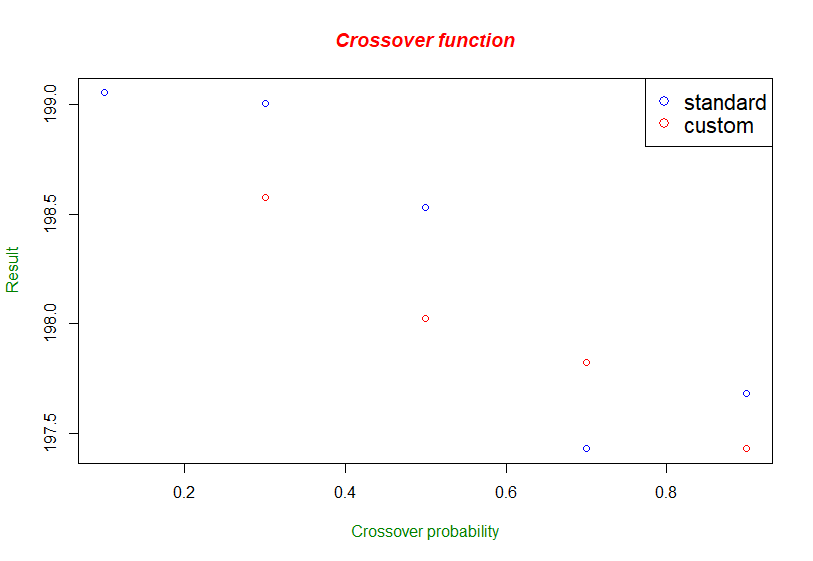
\includegraphics[scale=0.5]{custCrossover_pcross_result}
	\caption{Rezultat optymalizacji}
	\label{rys:fftFiltry}
\end{figure}

\begin{figure}[H]
	\centering
	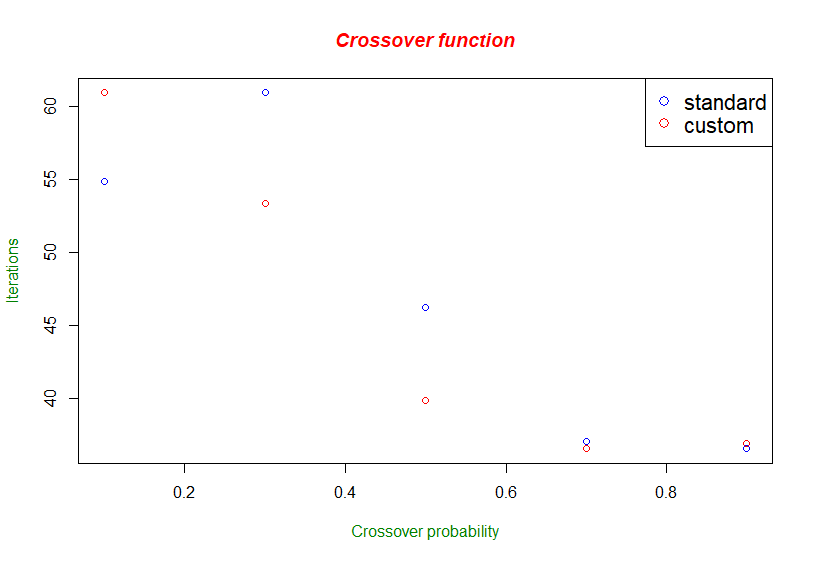
\includegraphics[scale=0.5]{custCrossover_pcross_iterations}
	\caption{Rezultat optymalizacji}
	\label{rys:fftFiltry}
\end{figure}


Zmiana ilości maksymalnej ilości iteracji

\begin{figure}[H]
	\centering
	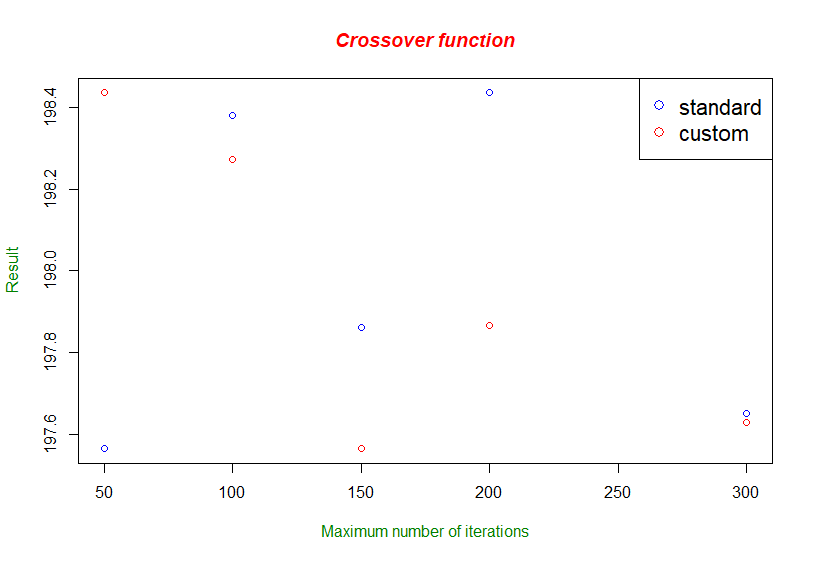
\includegraphics[scale=0.5]{custCrossover_maxIter_result}
	\caption{Rezultat optymalizacji}
	\label{rys:fftFiltry}
\end{figure}

\begin{figure}[H]
	\centering
	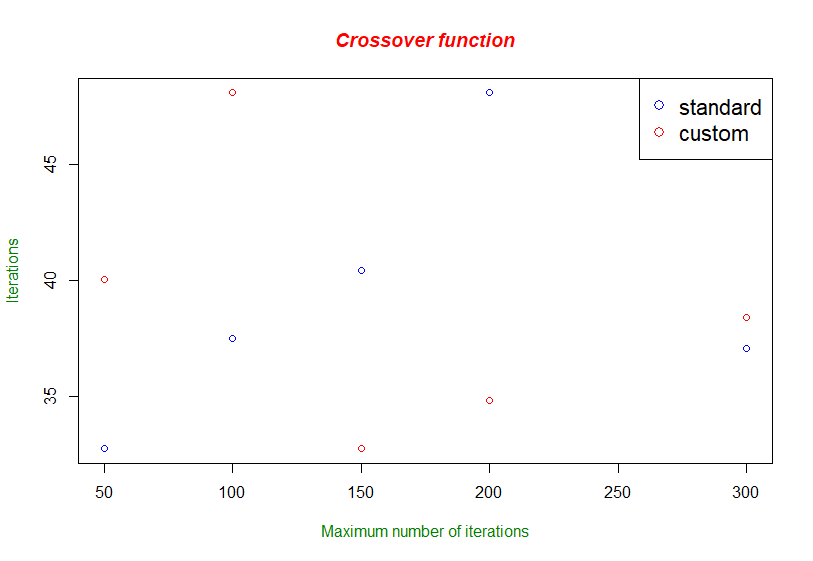
\includegraphics[scale=0.5]{custCrossover_maxIter_iterations}
	\caption{Rezultat optymalizacji}
	\label{rys:fftFiltry}
\end{figure}